% 可自定义论文时间戳 \today
% \year=2021
% \month=5
% \day=20

\documentclass{packages/sysuthesis} % 默认使用电子版（不填充空白页）。如果需要双面打印版，请注释掉本行并启用下一行
\usepackage{packages/sysucode}  % 在论文中使用代码
% 允许在长路径或单词中自动换行
\usepackage{xurl}
\usepackage[most]{tcolorbox} % 支持附录中的问答彩色框
\pgfplotsset{compat=1.18,compat/show suggested version=false} % 固定兼容版本并关闭提示信息
\setlength{\headheight}{13pt} % 消除 fancyhdr 的 headheight 告警
%%
% 论文相关信息
% 本文档中前缀"c-"代表中文版字段, 前缀"e-"代表英文版字段
% modifyer: 黄俊杰(huangjj27, 349373001dc@gmail.com)
% update date: 2017-04-13
%%

% 标题
% 论文题目应以简短、明确的词语恰当概括整个论文的核心内容,避免使用不常见的缩略词、缩写字。读者通过标题可大致了解毕业设计(论文)的内容、专业的特点和科学的范畴。中文题目一般不宜超过 24 个字,必要时可增加副标题。外文题目一般不宜超过 12 个实词

% 封面标题。由于技术所限，封面题目过长的划分交由用户您进行定夺
% 这也能让您的论文封面看起来更有美感
\covertitlefirst{编译原理}
\covertitlesecond{实验课第二次作业}

% Author:   Souler Ou
% 修改者:    欧一锋
% Date:     3/30/2018
% Mail:     ou@souler.cc
%如果英文标题过长可以使用此两项作为表三(答辩记录表)的标题。
% \etitlefirst{Dynamic 3D Generation and Physical Simulation}
% \etitlesecond{From Gaussian-Flow to PhysDreamer}

% 页眉标题
\ctitle{编译原理——实验第二次作业}

% 作者详细信息
% \author{林宏宇}
% \eauthor{Lin Hongyu}

\cauthor{林宏宇}    % 封面作者
\studentid{23320093}
\cschool{计算机学院}
\cmajor{计算机科学与技术}
\emajor{Computer Science and Technology}

% 指导老师
\cmentor{李文军}
% \ementor{Computer Graphics Course}

     % 论文相关信息
% 中文
\cabstract{
根据实验内容 \cite{lab02}, 在此次实验需要实现一个议程管理系统，此报告参照评分标准\cite{labeval02}，完成这份实验报告撰写并附上相应的实验报告说明。
本实验实现了一个基于命令行（CLI）的议程管理系统（Agenda），使用 Java 语言并采用面向对象设计。系统提供 `register`、`add`、`query`、`delete`、`clear`、`batch`、`quit` 等命令，支持交互式与批处理模式。核心采用单例的 `AgendaManager` 负责命令解析、鉴权与业务调度，命令通过 `Command` 接口实现分发；会议信息以内存结构（`Map<String, User>` 与 `List<Meeting>`）存储，时间处理基于 `java.time`。实现要点包括时间格式校验与解析、时间重叠检测、标签唯一性校验与批处理逐行回放。为保证质量，编写了 JUnit5 单元测试并集成到构建脚本中。本实验强化了面向对象建模、错误处理与自动化测试的实践，为后续引入持久化与并发支持提供了基础。
}
\ckeywords{议程管理；Java；命令行；面向对象；单元测试；批处理}

     % 摘要内容

\begin{document}
% 论文前置部分
\frontmatter
\pagenumbering{Roman}
\makeUndergraduateCover    % 封面

\makecabstract                       
\newpage
\maketableofcontents        % 目录

% 论文主体部分
\mainmatter
% 引言

% 正文
\definecolor{codebg}{RGB}{248,249,250}
\definecolor{codeframe}{RGB}{220,223,228}
\definecolor{codekw}{RGB}{25,85,145}
\definecolor{codecm}{RGB}{90,125,90}
\definecolor{codestr}{RGB}{136,44,136}
% Java代码风格
\lstdefinestyle{cleanjava}{
  language=Java,
  basicstyle=\ttfamily\small,
  keywordstyle=\bfseries\color{codekw},
  commentstyle=\itshape\color{codecm},
  stringstyle=\color{codestr},
  backgroundcolor=\color{codebg},
  frame=single,
  rulecolor=\color{codeframe},
  framesep=6pt,
  numbers=left,
  numberstyle=\scriptsize\color{gray},
  numbersep=8pt,
  breaklines=true,
  breakatwhitespace=false,
  showstringspaces=false,
  keepspaces=true,
  tabsize=4,
  columns=fullflexible
}


\chapter{实验目的}
本实验实现一个基于命令行的议程管理系统（Agenda）。目标是通过面向对象设计与命令行交互实现系统的基本功能，熟悉需求分析、异常处理以及回归测试的编写与运行。
\begin{itemize}
  \item \textbf{面向对象设计实践}：通过类与包结构组织代码，体现封装、职责分离与低耦合。
  \item \textbf{命令行接口实现}：实现作业要求的交互式命令与批处理执行，便于测试与自动化验证。
  \item \textbf{健壮性与测试}：对输入与时间格式做校验，处理异常并输出友好错误信息；提供批处理用例支持回归测试。
\end{itemize}

\chapter{实验环境}
\textbf{编程语言}

Java（建议使用 JDK 1.5 及以上，源码使用了 `java.time` API）。

\textbf{开发工具}

可使用任意文本编辑器或 IDE（Eclipse、IntelliJ IDEA、VS Code 等）。仓内包含 `build.bat`、`run.sh` 与 `agenda.bat`，用于快速编译、JUnit测试与运行。

\chapter{项目组织}

\begin{itemize}
  \item src/：源代码目录，包含主程序与业务逻辑实现。
    \begin{itemize}
    \item \textbf{src/AgendaService.java}：程序入口，支持交互式与批处理两种模式（`-batch fileName`）。
    \item \textbf{src/agenda/AgendaManager.java}：命令解析与业务逻辑实现，管理用户与会议信息（内存存储）。已重构为单例（饿汉式）并采用命令分发机制。
    \item \textbf{src/agenda/User.java}：用户对象，维护参与与创建的会议列表，提供认证与查找接口。
    \item \textbf{src/agenda/Meeting.java}：会议对象，包含起止时间、标签、发起者与被约者，并提供重叠检测与格式化输出。
    \item \textbf{src/agenda/Command.java}：命令接口（Command 模式），用于解耦命令解析与执行，所有具体命令类均实现此接口。
    \item \textbf{src/agenda/RegisterCommand.java}：实现 `register` 命令的处理逻辑，负责校验参数并在全局用户表中新增用户。
    \item \textbf{src/agenda/AddCommand.java}：实现 `add` 命令，解析起止时间、校验格式与冲突、构造 `Meeting` 并将其添加到相关用户。
    \item \textbf{src/agenda/QueryCommand.java}：实现 `query` 命令，解析时间区间并筛选该用户在区间内的会议，按起始时间排序后输出。
    \item \textbf{src/agenda/DeleteCommand.java}：实现 `delete` 命令，验证调用者为会议创建者并删除会议，同时清理另一方的引用。
    \item \textbf{src/agenda/ClearCommand.java}：实现 `clear` 命令，删除调用者创建的所有会议并移除相应引用。
    \item \textbf{src/agenda/BatchCommand.java}：实现 `batch` 命令，用于读取并逐行执行批处理文件中的命令，支持注释与回显。
    \item \textbf{src/agenda/QuitCommand.java}：实现 `quit` 命令，打印退出提示并终止 JVM，用于交互式退出。
    \item \textbf{src/agenda/AgendaManagerTest.java}：JUnit5 单元测试类，包含对 `AgendaManager` 单例和 `register` 命令的自动化测试（由 `./build.sh` 执行）。
    \end{itemize}
  \item doc/：javadoc文档目录。
  \item bin/：编译输出目录，存放编译后的 `.class` 文件。
  \item build.sh / build.bat：编译脚本，并进行 JUnit 测试。
  \item run.sh / agenda.bat：运行脚本，支持交互式与批处理模式。
  \item test.pdf：测试用例与结果截图，包含交互式与批处理的示例输入输出。
  \item design.pdf：设计文档，包含 UML 类图与时序图，说明系统设计与模块划分。
\end{itemize}


\chapter{建模与设计}
\section{总体架构}

本系统采用三层的简化架构：表示层（命令行入口）、业务逻辑层（管理器与命令分发）、领域模型层（用户与会议）。程序入口为 \path{AgendaService.java}，负责交互式或批处理两种运行模式；核心业务由单例的 \path{agenda/AgendaManager.java} 负责（命令解析、鉴权、数据存储与调度）；领域对象为 \path{agenda/User.java} 与 \path{agenda/Meeting.java}。命令采用命令模式（实现 \path{agenda/Command.java} 接口），具体命令类（如 \path{RegisterCommand.java}、\path{AddCommand.java} 等）在 \texttt{AgendaManager} 的构造中注册。

存储采用内存结构：在 \texttt{AgendaManager} 中使用一个 \texttt{Map<String, User>} 保存注册用户（以用户名为键）。时间处理基于 \texttt{java.time}，使用的时间格式为 \path{yyyy-MM-dd_HH:mm}（代码中由常量格式化器维护）。批处理由 \path{AgendaManager.processBatch} 实现，按行回显并继续处理，遇错不终止整个批次。

\section{UML}
\begin{figure}
\centering
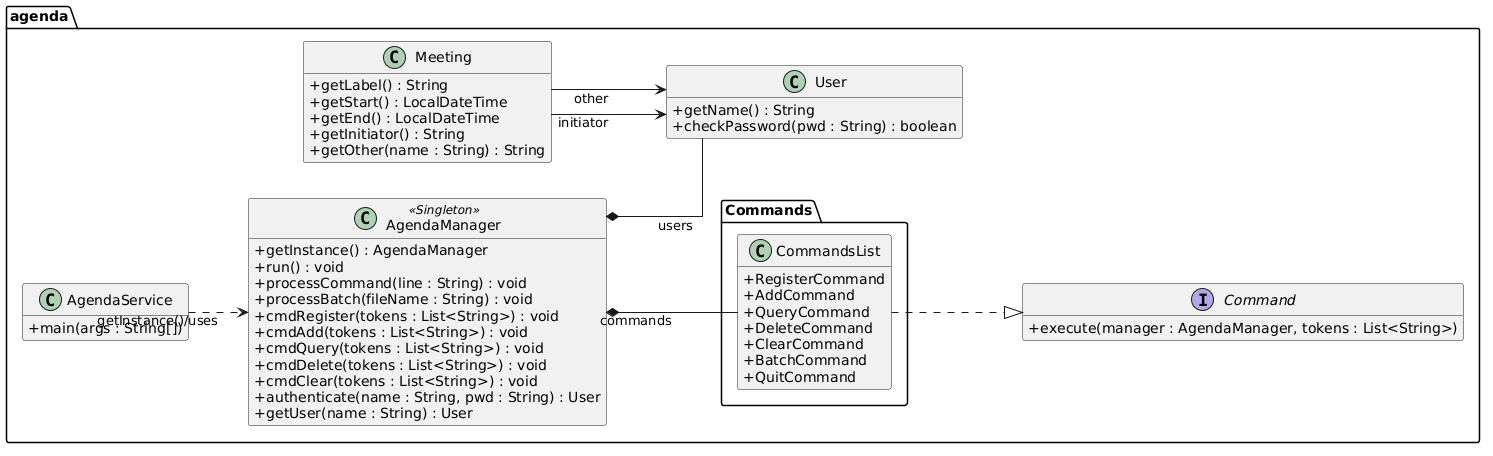
\includegraphics[width=\textwidth]{image/UML.png}
\caption{UML 类图}
\end{figure}
\section{数据模型与不变式}

领域模型由两个主要类构成：
\begin{itemize}
  \item \texttt{User}：属性包含用户名（\texttt{name}）、密码（\texttt{password}）、参与的会议列表（\texttt{meetingsAll}）和创建的会议列表（\texttt{meetingsCreated}）。提供的操作包括认证（\texttt{checkPassword}）、添加/删除会议（\texttt{addMeeting}, \texttt{removeMeeting}）、管理创建的会议（\texttt{addMeetingCreated}, \texttt{removeCreated}）以及按标签查找创建的会议（\texttt{findCreatedByLabel}）。
  \item \texttt{Meeting}：属性包含标签/标识（\texttt{label}）、起始时间（\texttt{start}）、终止时间（\texttt{end}）、发起者（\texttt{initiator}）和另一方（\texttt{other}）。提供时间重叠判断（\texttt{overlaps}）、为特定用户格式化输出（\texttt{formatForUser}）等方法。
\end{itemize}

关键不变式（在代码中受约束并通过调用路径维护）：
\begin{itemize}
  \item 用户名唯一：注册时在 \texttt{AgendaManager.users} 中检查（若存在则拒绝注册）。
  \item 会议时间有序：任何会议满足 \(start < end\)，在添加时由 \texttt{AgendaManager.cmdAdd} 验证。\newline
  \item 标签在创建者范围内唯一：发起者不能重复使用同一标签（由 \texttt{User.hasCreatedLabel} 检查）。
  \item 参与者均为已注册用户：添加会议前检查另一方是否存在，否则返回 \texttt{Error: other user not found}。
  \item 无重叠：对任一用户，其参与的会议集合中任意两会时间段不应重叠；添加时通过遍历该用户会议并调用 \texttt{Meeting.overlaps} 检查（若冲突则返回 \texttt{Error: time overlap}）。
  \item 权限约束：只有会议的发起者（initiator）可删除该会议（在发起者的 \texttt{meetingsCreated} 列表中查找标签以确认）。
  \item 数据一致性：添加/删除操作同时在双方的参与列表中保持对称（添加时在双方调用 \texttt{addMeeting}；删除/清除时在另一方调用 \texttt{removeMeeting}）。
\end{itemize}

\section{关键算法}

算法主要集中在时间解析、冲突检测与查询上，代码实现要点如下：
\begin{itemize}
  \item 时间解析：使用 \texttt{LocalDateTime.parse(..., FMT)}。FMT 由 \path{DateTimeFormatter.ofPattern} 指定，格式为 \path{yyyy-MM-dd_HH:mm}。
  解析失败时，程序输出错误提示：\texttt{Error: bad time format}。
  \item 冲突检测（时间重叠）：对于待插入时间区间 $[s,e)$，对目标用户的每个已有会议 $[s_i,e_i)$ 调用
  \begin{equation*}
    \text{overlaps} \iff s < e_i \; \text{and} \; s_i < e
  \end{equation*}
  这是由方法 \texttt{Meeting.overlaps} 实现的；算法复杂度为 $O(k)$，其中 $k$ 为该用户的会议数。
  \item 查询：遍历用户的所有会议，筛选出与查询区间重叠的会议（同上），然后按起始时间用 \path{Comparator.comparing(Meeting::getStart)} 排序，复杂度为 $O(n\\log n)$（$n$ 为匹配到的会议数，排序耗时占主导）。
  \item 标签唯一性与创建者校验：通过遍历发起者的 \texttt{meetingsCreated} 列表完成，复杂度为 $O(c)$（$c$ 为创建的会议数）。
\end{itemize}

\section{业务设计}

系统按命令驱动，主要命令及其语义（与实现对应）：
\begin{itemize}
  \item \texttt{register [userName] [password]}：在 \path{AgendaManager.cmdRegister} 中实现，进行用户名唯一性检查并在成功时创建 \texttt{User}。
  \item \texttt{add [userName] [password] [other] [start] [end] [title]}：在 \path{AgendaManager.cmdAdd} 中实现，完成认证、参数解析、被约者存在性检查、时间合法性检查、标签唯一性检查与重叠检测，成功后在双方维护的会议列表中添加 \texttt{Meeting}。
  \item \texttt{query [userName] [password] [start] [end]}：在 \texttt{AgendaManager.cmdQuery} 中实现，筛选并按起始时间排序输出匹配会议。
  \item \texttt{delete [userName] [password] [meetingId]}：在 \texttt{AgendaManager.cmdDelete} 中实现，仅允许发起者删除，同时在另一方移除对应引用。
  \item \texttt{clear [userName] [password]}：在 \texttt{AgendaManager.cmdClear} 中实现，删除该用户创建的所有会议并同步更新对方列表。
  \item \texttt{batch [fileName]}：在 \texttt{AgendaManager.processBatch} 中实现，逐行回显并执行，忽略空行与以 \texttt{\#} 开头的注释行；遇到 I/O 异常时打印提示并继续或终止（取决于异常类型）。
\end{itemize}


错误处理策略以明确的用户可读错误提示为主（例如 \texttt{Error: authentication failed}、\texttt{Error: time overlap} 等），并保证批处理模式下遇到单条命令错误不会中断整个批次的执行，便于回放与调试。

\section{面向对象建模与设计}
\subsection{业务逻辑层建模}

\texttt{AgendaManager} 负责命令解析与调度、全局用户表维护、鉴权与跨对象的事务性操作（例如在删除会议时同时更新两个用户的列表）。其实现把命令行为委托给实现了 \texttt{Command} 接口的具体命令对象，降低了管理器类的复杂度并便于单元测试。

\subsection{表示层建模}

表示层目前为基于命令行的简单实现，由 \path{AgendaService.main} 启动。交互式模式由 \path{AgendaManager.run} 提供循环读取与提示（比如打印 \texttt{\$} 提示符）。批处理模式由启动参数触发并调用 \texttt{processBatch}。

\subsection{对象属性及其类型设计}

主要字段示例：
\begin{itemize}
  \item \texttt{User.name}：\texttt{String}，身份标识。
  \item \texttt{User.password}：\texttt{String}，用于简单认证（示例实现中为明文比较）。
  \item \texttt{User.meetingsAll} / \texttt{User.meetingsCreated}：\texttt{List<Meeting>}，分别记录参与与创建的会议。
  \item \texttt{Meeting.start}, \texttt{Meeting.end}：\texttt{LocalDateTime}，用于精确比较与格式化输出。
\end{itemize}

\subsection{对象操作及其接口设计}

通过将命令行为抽象为 \texttt{Command.execute(AgendaManager, List<String>)}，实现了操作的统一入口与扩展点；领域对象提供必要的最小接口（如 \texttt{getMeetings()}, \texttt{addMeeting()}, \texttt{findCreatedByLabel()} 等），管理器使用这些接口完成更高层的业务流程。

\subsection{访问控制设计及其他}

当前访问控制策略为基于用户名/密码的简单鉴权，所有需要用户身份的命令均调用 \texttt{AgendaManager.authenticate} 完成密码校验；删除会议等敏感操作在业务上进一步校验发起者身份（通过在创建列表中查找标签）。对于真实生产系统，应替换为更安全的认证与持久化方案。

\subsection{多态性与表示独立性分析}

\textbf{多态性（Polymorphism）}
项目通过定义 \texttt{Command} 接口（见 \path{src/agenda/Command.java}）并让各具体命令类（如 \path{RegisterCommand.java}、\path{AddCommand.java} 等）实现该接口，利用多态在运行时决定命令行为。\texttt{AgendaManager} 在构造时将命令注册到一个 \texttt{Map<String, Command>} 中，接收到输入后只需通过键查找并调用 \texttt{command.execute(this, tokens)} 完成分发。这一做法将解析/分发与具体执行解耦，便于新增命令、单元测试和行为替换。

\textbf{表示独立性（Representation Independence）}
表示独立性指接口（行为）与具体内部表示之间的隔离，外部通过接口与对象交互而不依赖其内部数据结构。项目在分层上已有较好基础：命令行表示层（\texttt{AgendaService}）与业务层（\texttt{AgendaManager}）分离，且领域对象 \texttt{Meeting} 使用 \texttt{LocalDateTime} 封装时间并通过 \texttt{formatForUser} 统一输出格式，这些都有利于保持表示独立性。

\section{GoF 设计模式}

本项目在若干位置采用了典型的设计模式以提高可维护性。

\textbf{Singleton（单例）}
\texttt{AgendaManager} 采用饿汉式单例实现（\texttt{private static final AgendaManager INSTANCE = new AgendaManager();} + 私有构造 + \texttt{public static AgendaManager getInstance()}）。单例保证了全局的用户表与命令注册只有一个共享实例，简化了测试与程序入口管理，但在并发或需要多实例隔离的场景下需要调整或引入依赖注入。

\textbf{Command（命令）}
通过定义 \texttt{Command} 接口并在管理器构造时把具体命令对象注册到一个 \texttt{Map<String, Command>} 中，\texttt{AgendaManager.processCommand} 只需查表并调用对应命令的 \texttt{execute} 方法即可完成请求分发。此模式便于新增命令、单独测试命令逻辑以及将命令与解析/调用解耦。


\chapter{功能说明与接口约定}
程序实现了作业中规定的命令格式与语义，命令名不区分大小写，参数区分大小写。

主要命令：
\begin{itemize}
  \item `register [userName] [password]`：注册新用户，用户名必须唯一。
  \item `add [userName] [password] [other] [start] [end] [title]`：添加会议；`title` 为会议标签（创建者范围内唯一）。
  \item `query [userName] [password] [start] [end]`：查询该用户在指定时间段内的所有会议（作为发起者或被约者）。
  \item `delete [userName] [password] [meetingId]`：删除由该用户创建且标签为 `meetingId` 的会议。
  \item `clear [userName] [password]`：清除该用户创建的所有会议。
  \item `batch [fileName]`：逐行执行批处理文件中的命令，支持注释行。
  \item `quit`：退出程序。
\end{itemize}

\chapter{测试}

\section{测试用例设计}

本报告的测试用例分为两类：基本功能测试与异常/错误测试。
基本功能测试覆盖注册（\texttt{register}）、添加（\texttt{add}）、查询（\texttt{query}）、删除（\texttt{delete}）和清除（\texttt{clear}）等正常流程，期望输出成功提示如 \texttt{Register success}、\texttt{Add success} 等。
异常测试包括：重复注册、预约未注册用户、时间格式错误、起止时间无效、时间重叠、认证失败、非创建者删除、删除不存在会议、批处理文件缺失等，期望输出相应错误提示（例如 \texttt{Error: user already exists}、\texttt{Error: other user not found}、\texttt{Error: bad time format}、\texttt{Error: start must be before end}、\texttt{Error: time overlap}、\texttt{Error: authentication failed}、\texttt{Error: meeting not found or not creator}、\texttt{Error: batch file not found: ...}）。
批处理模式会回显每条命令并输出结果，便于人工或脚本化核对。

\section{测试结果}

\textbf{基本功能测试用例：}

\begin{lstlisting}[style=cleanjava]
register alice 123
register bob 456
add alice 123 bob 2026-04-09_10:00 2026-04-09_11:00 TeamMeeting
query alice 123 2026-04-09_00:00 2026-04-10_00:00
delete alice 123 TeamMeeting
clear alice 123
quit
\end{lstlisting}

\begin{figure}[htbp]
\centering
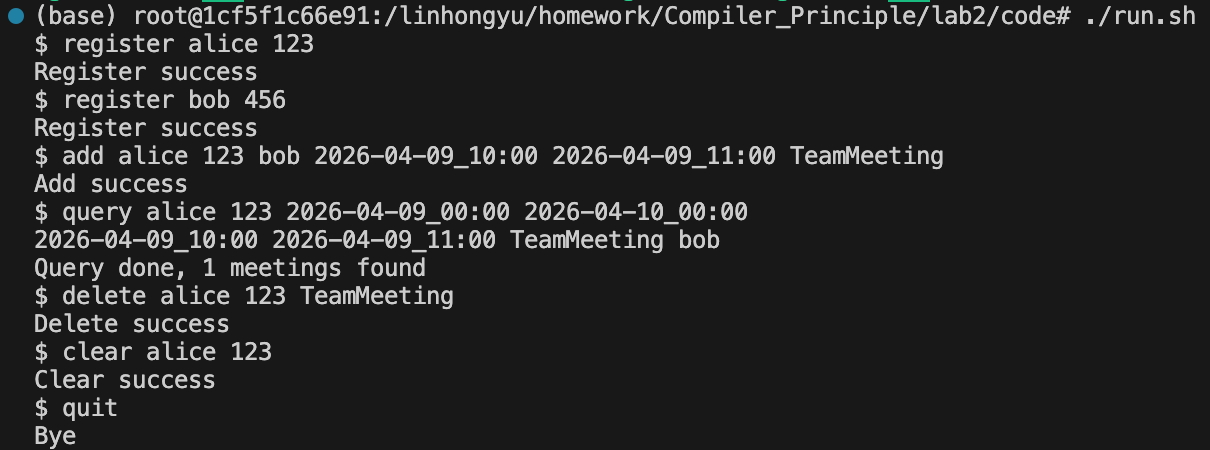
\includegraphics[width=0.85\textwidth]{image/test1.png}
\end{figure}

\textbf{批处理用例设计：}

\begin{lstlisting}[style=cleanjava]
register alice 123
register bob 456
add alice 123 bob 2026-04-09_10:00 2026-04-09_11:00 TeamMeeting
register alice 000
add alice 123 charlie 2026-04-09_12:00 2026-04-09_13:00 InvalidOther
add alice 123 bob 2026/04/09 12:00 2026/04/09 13:00 BadTimeFormat
add bob 456 alice 2026-04-09_14:00 2026-04-09_14:00 ZeroLength
add bob 456 alice 2026-04-09_10:30 2026-04-09_11:30 OverlapMeeting
query bob wrongpwd 2026-04-09_00:00 2026-04-10_00:00
delete bob 456 TeamMeeting
creator）
delete alice 123 NonExist
nonexist.txt）
batch nonexist.txt
query alice 123 2026-04-09_00:00 2026-04-10_00:00
delete alice 123 TeamMeeting
clear alice 123
quit
\end{lstlisting}

\begin{figure}[htbp]
\centering
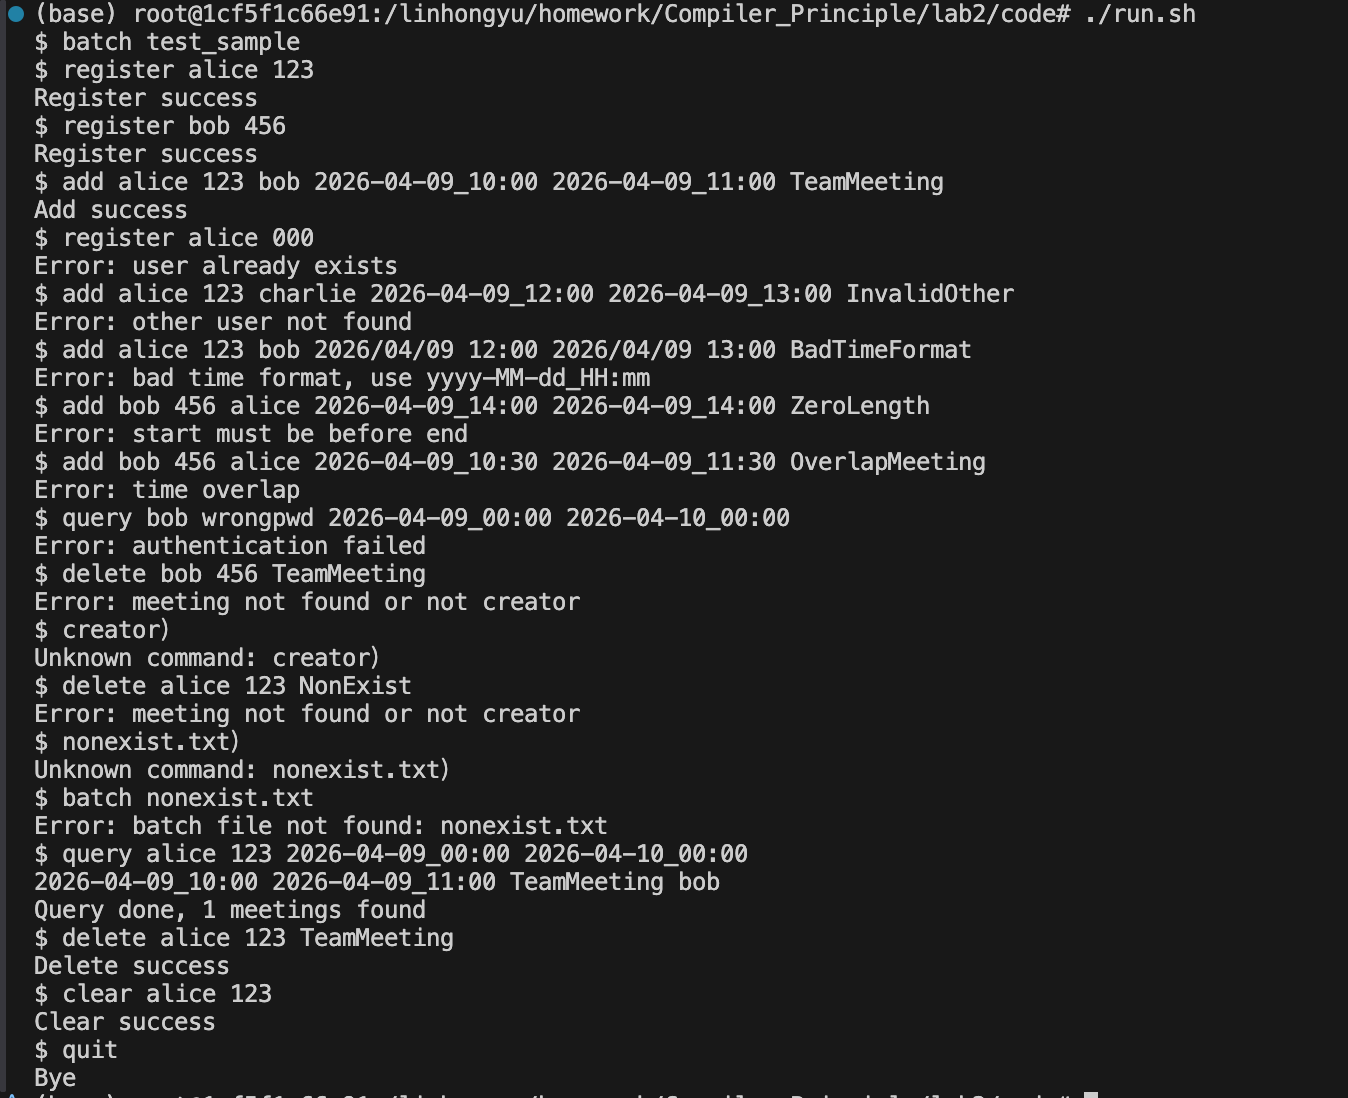
\includegraphics[width=0.9\textwidth]{image/test2.png}
\end{figure}


\section{单元测试（JUnit5）}

当前JUnit测试用例包括：
\begin{itemize}
  \item 单例一致性：验证 `AgendaManager.getInstance()` 返回相同实例（方法 `singletonInstanceIsSame`）。
  \item 注册命令功能：通过调用 `processCommand("register ...")` 验证用户被正确创建（方法 `registerCreatesUser`）。
\end{itemize}

\textbf{测试运行输出示例与说明}

\begin{lstlisting}[style=cleanjava]
Test run finished after 88 ms
[         4 containers found      ]
[         0 containers skipped    ]
[         4 containers started    ]
[         0 containers aborted    ]
[         4 containers successful ]
[         0 containers failed     ]
[         2 tests found           ]
[         0 tests skipped         ]
[         2 tests started         ]
[         0 tests aborted         ]
[         2 tests successful      ]
[         0 tests failed          ]
\end{lstlisting}
说明：
\begin{itemize}
  \item \textbf{Found test sources...}：构建脚本检测到测试文件并提示需将 JUnit jar 放到 `lib/`。
  \item \textbf{Compiling tests...}：测试源被编译到 `bin/`（编译会引入 JUnit jar 到类路径用于测试引擎）。
  \item \textbf{Running tests...}：调用 JUnit 控制台（`execute` 子命令）执行测试。
  \item \textbf{Register success}：这是程序在执行 `register` 命令时打印的正常输出（由 `AgendaManager.cmdRegister` 打印），说明命令逻辑已完成。
  \item JUnit 报告树（`JUnit Platform Suite` / `JUnit Jupiter` / `AgendaManagerTest`）：显示测试套件结构及每个 `@Test` 的执行结果（`✔` 表示通过）。
  \item 报告底部统计：列出执行的容器与测试数量与通过率，便于自动化判定（非零失败数应视为回归问题）。
\end{itemize}
JUnit单元测试总结：
\begin{itemize}
  \item 自动化验证关键行为（例如单例一致性与命令执行效果），便于在修改代码后快速回归检查。
  \item 与程序输出结合（如 `Register success`）可以同时验证业务逻辑的控制流与用户可见输出。
  \item 将测试集成到 `build.sh` 后，CI 或提交前钩子可直接调用脚本进行快速验证。
\end{itemize}


\chapter{自我评分参照}

本实验自我评分标准如下表所示，并对每一项在报告中的对应章节进行了标注：


\begin{table}[htbp]
	\centering
	\begin{tabular}{|p{5cm}|c|p{9cm}|}
	\hline
  评分项目 & 权重 & 报告对应章节 \\
  \hline 
  1. 基本功能需求 & 20\% & 见“功能说明与接口约定”与“测试” \\
  1.1 可运行的程序 & 20\% & 见运行脚本与“项目组织” \\
  2. 编程风格  & 15\% & 见源代码与报告中代码片段 \\
  2.1 标识符命名 & 5\% & 见“项目组织”与源码中的命名与注释 \\
  2.2 文档化注释 & 5\% & 见源码注释与本报告文档部分 \\
  2.3 程序版面 & 5\% & 见项目组织与代码格式 \\
  3. 面向对象建模与设计 & 40\% & 见“建模与设计”章节 \\
  3.1 业务逻辑层建模 & 10\% & 见“建模与设计” 业务逻辑层建模小节 \\
  3.2 表示层建模 & 15\% & 见“建模与设计” 表示层建模小节 \\
  3.3 对象属性及其类型设计 & 5\% & 见“建模与设计” 对象属性部分 \\
  3.4 对象操作及其接口设计 & 5\% & 见“建模与设计” 对象操作及其接口设计 \\
  3.5 访问控制设计及其他 & 5\% & 见“建模与设计” 访问控制设计与不变式部分 \\
  4. 实验报告 & 10\% & 本报告整体（章节索引见目录） \\
  4.1 实验报告内容 & 3\% & 见“建模与设计”与“测试” \\
  4.2 UML表示 & 5\% & 见“UML”章节 \\
  4.3 文档与源程序组织 & 2\% & 见“项目组织”章节 \\
  5. 其他 & 15\% & 见“改进建议”与“实验总结” \\
  5.1 程序包运用 & 3\% & 见项目包结构 \\
  5.2 异常处理 & 7\% & 见“业务设计”中的错误处理与批处理支持，以及“测试”中的异常用例 \\
  5.3 测试用例及测试结果 & 5\% & 见“测试”章节 \\
  \hline
\end{tabular}
\caption{评分项目与对应报告章节}
\label{tab:self-eval-map}
\end{table}


\chapter{实验总结}

\section{技术总结}
\begin{itemize}
  \item 系统实现与功能：实现了基于命令行的议程管理系统（Agenda），支持 `register`、`add`、`query`、`delete`、`clear`、`batch`、`quit` 等命令，支持交互式与批处理两种运行模式（由 `AgendaService` 启动，使用 `-batch` 参数触发批处理）。
  \item 架构与关键模块：系统按表示层（`AgendaService`）、业务层（单例 `AgendaManager`）和领域模型（`User`、`Meeting`）分层；命令通过 `Command` 接口分发，具体命令类在管理器构造时注册，便于扩展与单独测试。
  \item 关键算法与实现要点：时间解析使用 `LocalDateTime.parse(..., FMT)`，其中 FMT 由 `DateTimeFormatter.ofPattern("yyyy-MM-dd\_HH:mm")` 指定；时间重叠判断采用 $s<e_i\land s_i<e$；查询先按重叠关系筛选再按起始时间排序（复杂度 $O(n\log n)$），冲突检测为对用户会议列表的线性扫描（$O(k)$）。
  \item 数据一致性与不变式：实现中通过在添加/删除操作中同时更新双方的会议列表来保证一致性；代码路径上维护用户名唯一、`start<end`、创建者范围内标签唯一、参与者必须已注册等不变式。
  \item 错误处理与批处理策略：对时间格式、参数完整性和权限做出明确的用户可读错误提示（例如 `Error: bad time format`、`Error: time overlap`）；`AgendaManager.processBatch` 实现逐行回显并在单条命令出错时继续执行，便于回放和自动化验证。
  \item 测试与验证：已编写 JUnit5 单元测试（如单例一致性与注册流程），并将测试集成到构建脚本（`build.sh`），同时通过批处理示例脚本验证典型正常与异常场景。
\end{itemize}

\section{实验收获}
\begin{itemize}
  \item 面向对象与建模实践：通过将业务拆分为 `AgendaManager`、`User` 与 `Meeting` 等领域对象，实践了封装、单一职责与低耦合的设计原则。
  \item 设计模式应用：在实践中体会到单例（`AgendaManager`）和命令模式（`Command`）对集中管理、扩展性与测试友好的作用。
  \item 时间与边界处理能力：掌握了 `java.time` 的解析、比较与格式化技巧，并理解时间边界与重叠检测对业务正确性的关键作用。
  \item 工程化与测试流程：通过批处理回放、JUnit 单元测试和构建脚本，增强了面向回归测试的开发流程与可重复性验证能力。
\end{itemize}

\section{心得体会}
先做充分的领域建模并把关键不变式在设计阶段写清楚，可以显著减少实现与调试时的返工；清晰的错误提示与批处理回放机制极大提升了问题定位与回归验证效率。
\newclearpage
% \include{content/chap02}
% \newclearpage

% 结语

% 附录部分
\backmatter
% 参考文献. 因不需要纳入章节目录, 故放入附录部分
% 实际上参考文献是属于论文主体部分
\makereferences

% 附录
{
    \appendix
    \include{appendix1}
    \newclearpage
}

% \include{content/ack}    % 致谢
\end{document}
